\thispagestyle{lichsutoanhocnone}
\pagestyle{lichsutoanhoc}
\graphicspath{{../lichsutoanhoc/pic/}}
\everymath{\color{lichsutoanhoc}}
\blfootnote{$^*$\color{lichsutoanhoc}Dịch theo https://mathshistory.st-andrews.ac.uk/Biographies/Noether\_Emmy/}
\blfootnote{$^1$\color{lichsutoanhoc}Đại học Sư phạm Hà Nội.}
\begingroup
\AddToShipoutPicture*{\put(0,616){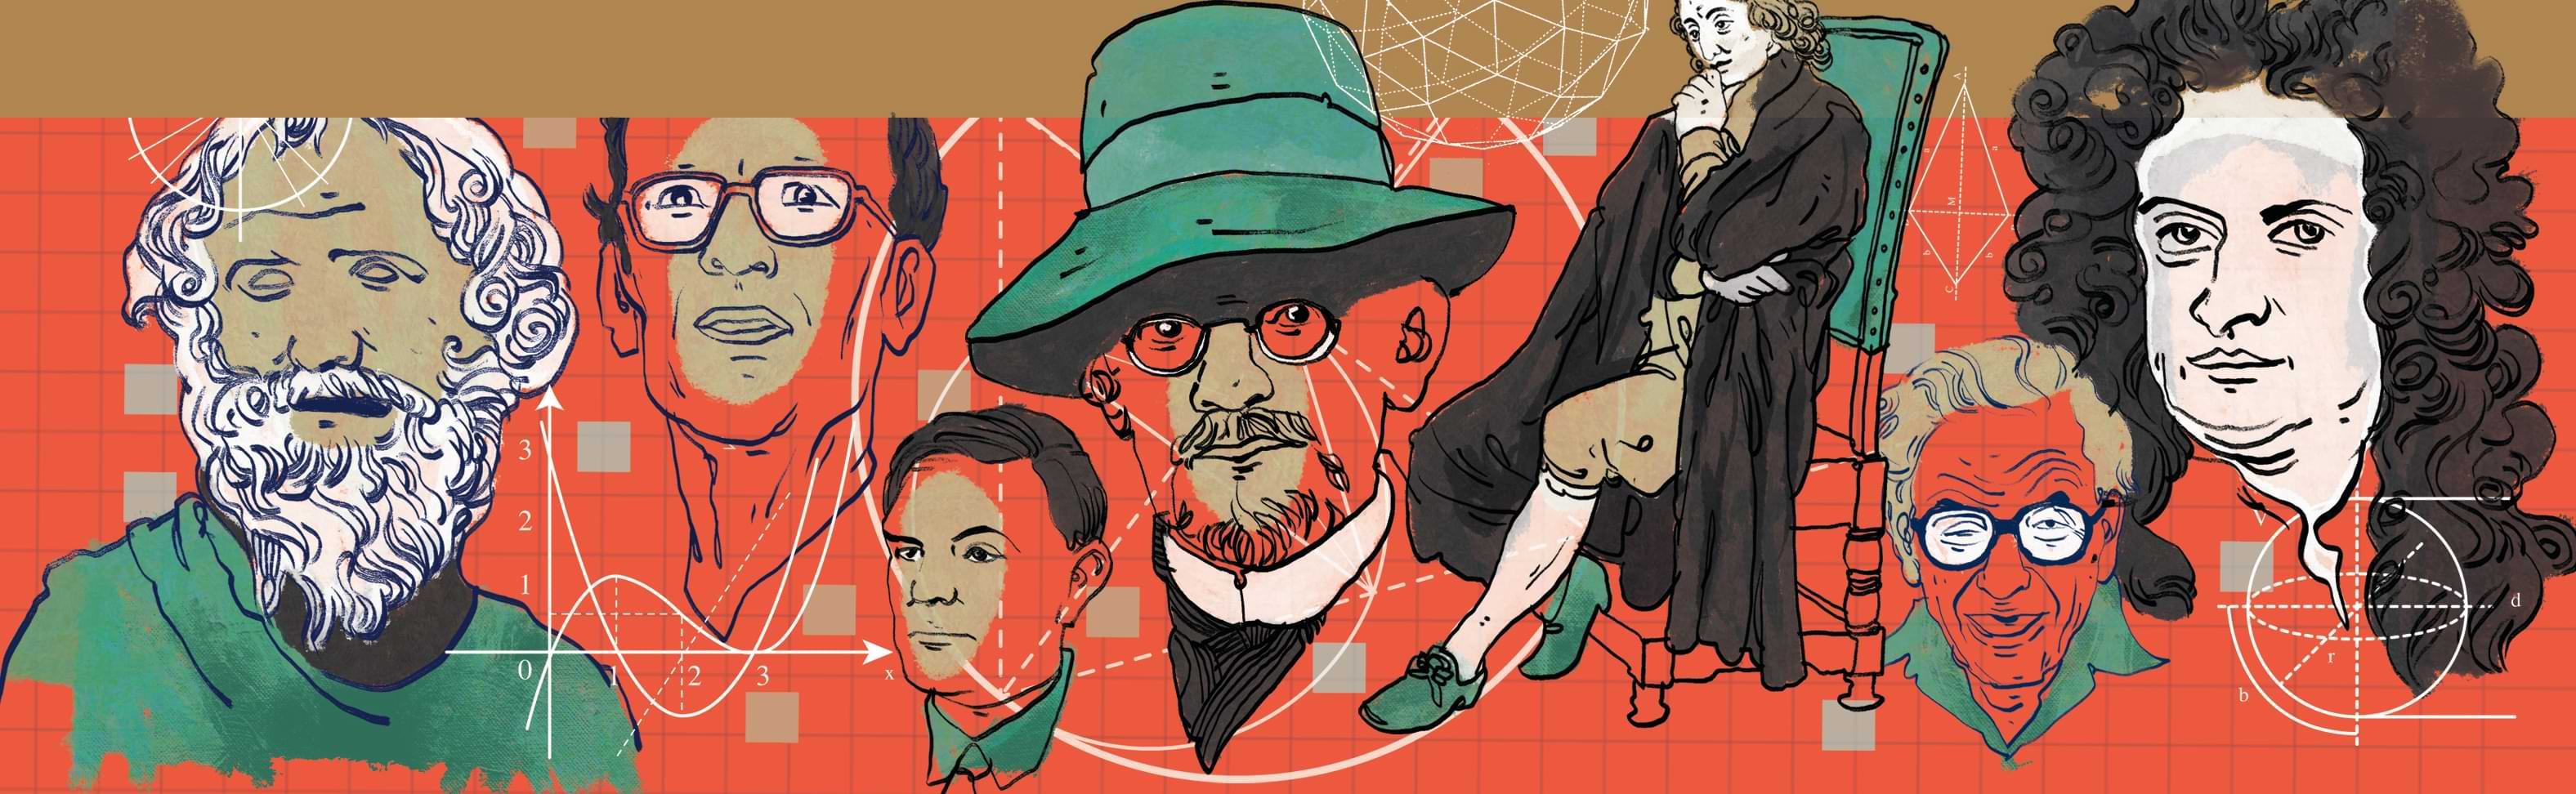
\includegraphics[width=19.3cm]{../bannerlichsu}}}
\AddToShipoutPicture*{\put(78,552){
\includegraphics[scale=1]{../tieude4.pdf}}}
\centering
\endgroup

\vspace*{160pt}

	``\textit{Phương pháp của tôi, quả thật là phương pháp của làm việc và suy nghĩ, 
	đó chính là lý do vì sao chúng len lỏi vào mọi nơi trong cuộc sống một cách ẩn danh}."
\begin{multicols}{2}
		\begin{figure}[H]
%		\vspace*{5pt}
		\centering
		\captionsetup{labelformat= empty, justification=centering}
		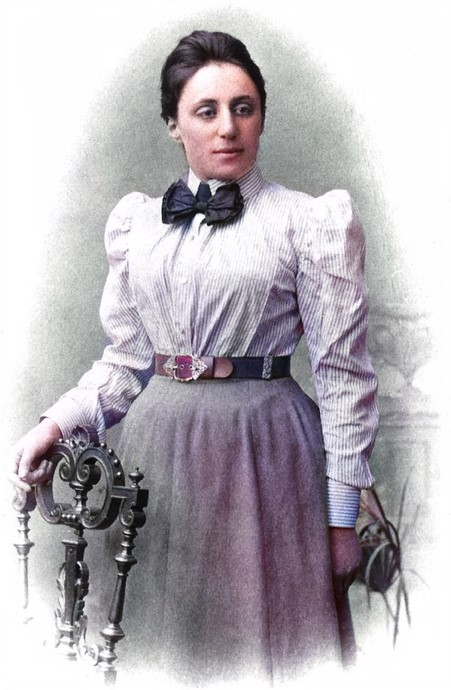
\includegraphics[width= 0.45\linewidth]{1a}
		\caption{\small\textit{\color{lichsutoanhoc}Emmy Amalie Noether ($1882-1935$).}}
		\vspace*{-10pt}
	\end{figure}
	Cha của Emmy Noether, Max Noether, là một nhà toán học nổi tiếng và là giáo sư tại Erlangen nhưng ông xuất thân từ một gia đình buôn bán đồ sắt thép. Mẹ cô là Ida Amalia Kaufmann ($1852-1915$), xuất thân từ một gia đình giàu có ở Cologne. Cha mẹ của Emmy đều có nguồn gốc Do Thái và người đọc có thể ngạc nhiên về điều này vì Noether không phải là tên Do Thái. Do đó, chúng ta nên giải thích điều này đã xảy ra như thế nào, đồng thời đưa ra một số thông tin về tổ tiên của Emmy Noether. Ông nội của Max Noether là Elias Samuel, người sáng lập một doanh nghiệp ở Bruchsal. Elias có chín người con,  một người con trai trong số đó là  Hertz Samuel. Năm $1809$, bang Baden ban hành Sắc lệnh Khoan dung yêu cầu người Do Thái lấy tên tiếng Đức. Elias Samuel chọn họ Nöther, trở thành Elias Nöther, nhưng cũng đổi tên các con mình, đặt cho Hertz cái tên Hermann. Khi được mười tám tuổi, Hermann Nöther rời quê hương Bruchsal và theo học thần học tại Đại học Mannheim. Sau đó vào năm $1837$, cùng với anh trai Joseph, ông thành lập một cơ sở kinh doanh bán buôn đồ sắt. Hermann Nöther và vợ Amalia có năm người con, người thứ ba là Max. Hai đứa trẻ lớn hơn Max là Sarah (sinh ngày $6$ tháng $11$ năm $1839$) và Emil. Điều đáng lưu ý ở điểm này là doanh nghiệp bán buôn sắt Nöther vẫn là một công ty gia đình trong đúng một trăm năm, cho đến khi Đức Quốc xã loại bỏ các gia đình Do Thái khỏi hoạt động kinh doanh của chính họ vào năm $1937$. Ta có một lưu ý cần thiết ở điểm này. Mặc dù họ của Max được ông nội của Max chọn là Nöther nhưng Max và gia đình ông  luôn sử dụng dạng Noether (ngoại trừ trên giấy chứng nhận đám cưới của Max có xuất hiện dạng Nöther).
	\vskip 0.05cm
	Emmy là con cả trong gia đình có bốn người con, ba người em nhỏ hơn là đều là con trai. Alfred Noether ($1883-1918$) nghiên cứu hóa học và nhận bằng tiến sỹ tại Erlangen năm $1909$. Tuy nhiên, sự nghiệp của ông rất ngắn ngủi vì ông qua đời $9$ năm sau đó. Fritz Noether ($1884-1941$) trở thành nhà toán học ứng dụng. Tuy nhiên, là một người Do Thái, ông không thể làm việc và phải rời nước Đức vào năm $1937$. Ông được bổ nhiệm làm giáo sư tại Đại học Tomsk ở Liên Xô nhưng bị buộc tội có hành động chống nhà nước  Xô Viết, ông bị kết án tử hình và bị xử bắn. Ông được Tòa án Tối cao Liên Xô tuyên vô tội vào năm $1988$. Gustav Robert Noether ($1889-1928$) suốt đời có sức khỏe kém. Ông bị thiểu năng trí tuệ, dành phần lớn cuộc đời trong viện dưỡng lão và chết trẻ. Ngôi trường đầu tiên Emmy theo học là ở Fahrstrasse. Auguste Dick viết trong [$2$]:
	\vskip 0.05cm
	\textit{Emmy không có vẻ gì đặc biệt khi còn nhỏ. Chơi đùa cùng các bạn trong sân trường ở Fahrstrasse, có lẽ cô ấy không đặc biệt đáng chú ý -- một cô bé cận thị, có vẻ ngoài giản dị, mặc dù không phải là không có duyên. Các giáo viên và bạn cùng lớp của cô biết đến Emmy như một đứa trẻ thông minh, thân thiện và dễ mến. Cô ấy nói hơi ngọng và là một trong số ít người tham gia các lớp học về đạo Do Thái.}
	\vskip 0.05cm
	Sau khi học tiểu học, Emmy Noether theo học tại Städtische Höhere Töchter Schule trên Friedrichstrasse ở Erlangen từ năm $1889$ đến năm $1897$. Cô sinh ra trong ngôi nhà gia đình ở Hauptstrasse $23$ và sống ở đó cho đến giữa thời gian học trung học, vào năm $1892$, gia đình chuyển đến một căn hộ lớn hơn ở Nürnberger Strasse $32$. Ở trường trung học, cô học tiếng Đức, tiếng Anh, tiếng Pháp, số học và được học piano. Cô thích khiêu vũ và mong chờ những bữa tiệc cùng con cái của các đồng nghiệp đại học của cha cô. Ở giai đoạn này, mục tiêu của cô là trở thành một giáo viên ngôn ngữ và sau khi học thêm tiếng Anh và tiếng Pháp, cô đã tham gia các kỳ thi của bang Bavaria và vào năm $1900$, cô trở thành giáo viên được cấp chứng chỉ dạy tiếng Anh và tiếng Pháp tại các trường nữ sinh ở Bavaria. Cô được điểm ``rất giỏi" trong các kỳ thi, mảng yếu nhất lại là việc giảng dạy trên lớp của cô.
	\vskip 0.05cm
	Tuy nhiên Noether chưa bao giờ trở thành giáo viên ngôn ngữ. Thay vào đó, cô quyết định đi theo con đường khó khăn đối với một phụ nữ thời đó và học toán ở trường đại học. Phụ nữ được phép học tại các trường đại học Đức một cách không chính thức và mỗi giáo sư phải cấp phép cho khóa học của mình. Noether được phép tham gia các khóa học tại Đại học Erlangen trong thời gian từ $1900$ đến $1902$. Cô là một trong hai sinh viên nữ duy nhất tham gia các khóa học tại Erlangen và, ngoài các khóa học toán, cô tiếp tục quan tâm đến các ngôn ngữ được dạy bởi một giáo sư về La Mã học và bởi một nhà sử học. Đồng thời, cô cũng chuẩn bị tham gia một kỳ thi cho phép sinh viên vào bất kỳ trường đại học nào. Sau khi vượt qua kỳ thi trúng tuyển ở Nürnberg vào ngày $14$ tháng $7$ năm $1903$, cô đã đến Đại học Göttingen. Trong thời gian $1903-04$, cô đã tham dự các bài giảng của Karl Schwarzschild, Otto Blumenthal, David Hilbert, Felix Klein và Hermann Minkowski. Một lần nữa, cô không được phép trở thành một sinh viên trúng tuyển chính thức mà chỉ được phép ngồi giảng bài. Sau một học kỳ tại Göttingen, cô trở lại Erlangen.
	\vskip 0.05cm
	Tại thời điểm này, các quy tắc đã được thay đổi và học sinh nữ được phép trúng tuyển trên cơ sở bình đẳng với nam giới. Ngày $24$ tháng $10$ năm $1904$, Noether trúng tuyển tại Erlangen, nơi bây giờ cô chỉ học toán. Năm $1907$, cô được cấp bằng tiến sỹ sau khi làm việc dưới sự hướng dẫn của Paul Gordan. Bài kiểm tra miệng diễn ra vào thứ Sáu ngày $13$ tháng $12$ và cô đã được trao bằng ``summa cum laude". Định lý cơ bản của Hilbert năm $1888$ đã đưa ra kết quả tồn tại tính hữu hạn của các bất biến trong $n$ biến. Tuy nhiên, Gordan đã áp dụng cách tiếp cận mang tính xây dựng và xem xét các phương pháp mang tính xây dựng để đạt được kết quả tương tự. Luận án tiến sỹ của Noether tuân theo cách tiếp cận mang tính xây dựng này của Gordan và liệt kê các hệ thống gồm $331$ dạng hiệp biến. Colin McLarty viết trong [$4$] rằng
	\vskip 0.05cm
	\textit{Luận án của cô năm $1908$ với Gordan theo đuổi một phép tính khổng lồ đã từng làm Gordan bối rối bốn mươi năm trước và ngay cả Noether cũng không thể hoàn thành được. Theo như tôi biết thì chưa có ai từng hoàn thành nó hoặc thậm chí đã từng kiểm tra nó như cô ấy đã làm. Vào thời điểm đó, nó đã lỗi thời, là một nhân chứng cho sự cô lập dễ chịu của Erlangen và  nó đã không tận dụng được công trình của chính Gordan xây dựng dựa trên ý tưởng của Hilbert.}
	\vskip 0.05cm
	Sau khi hoàn thành bằng tiến sỹ, quá trình bình thường để đạt được một vị trí học thuật sẽ là luận án tiến sỹ khoa học. Tuy nhiên con đường này không dành cho phụ nữ nên Noether vẫn ở lại Erlangen, giúp đỡ cha cô, một người đặc biệt vì sự ốm yếu bệnh tật của mình nên rất biết ơn sự giúp đỡ của con gái ông. Noether cũng thực hiện nghiên cứu của riêng mình, đặc biệt là cô chịu ảnh hưởng của Ernst Fischer, người kế nhiệm Gordan làm trưởng khoa toán học khi ông nghỉ hưu năm $1911$. Noether viết về ảnh hưởng của Fischer:
	\vskip 0.05cm
	\textit{Trên hết, tôi mang ơn ông E. Fischer, người đã thúc đẩy tôi nghiên cứu đại số trừu tượng từ quan điểm số học, và đây vẫn là ý tưởng chủ đạo cho tất cả công việc sau này của tôi.}
	\vskip 0.05cm
	Ảnh hưởng của Fischer đã đưa Noether hướng tới cách tiếp cận trừu tượng của Hilbert đối với chủ đề này và tránh xa cách tiếp cận mang tính xây dựng của Gordan. Điều này rất quan trọng đối với sự phát triển của cô với tư cách là một nhà toán học bởi  Gordan, mặc dù có những thành tựu đáng chú ý nhưng cũng có những hạn chế của ông. Cha của Noether, Max Noether, nói về Gordan (xem [$1$]):
	\vskip 0.05cm
	\textit{Gordan không bao giờ có thể đánh giá đúng sự phát triển của các khái niệm cơ bản; ngay cả trong các bài giảng của mình, ông ấy đã hoàn toàn tránh xa mọi định nghĩa cơ bản về bản chất khái niệm, thậm chí cả định nghĩa về giới~hạn.}
	\vskip 0.05cm
	Danh tiếng của Noether tăng lên nhanh chóng khi các ấn phẩm của cô xuất hiện. Năm $1908$, cô được bầu vào Circolo Matematico di Palermo, sau đó vào năm $1909$, cô được mời trở thành thành viên của Deutsche Mathematiker--Vereinigung và cùng năm đó, cô được mời phát biểu tại cuộc họp thường niên của Hiệp hội ở Salzburg. Cô đã giảng bài \textit{Zur Invariantentheorie der Formen von $n$ Variabeln}. Năm $1913$, cô giảng dạy ở Vienna, một lần nữa tại một cuộc họp của Deutsche Mathematiker--Vereinigung. Bài giảng của cô trong dịp này là \textit{Über Reasone Funktionenkörper}. Khi ở Vienna cô đã đến thăm Franz Mertens và trao đổi thảo luận về toán học với ông. Một trong những người cháu trai của Mertens nhớ lại chuyến viếng thăm của Noether (xem [$2$]):
	\vskip 0.05cm
	\textit{\ldots mặc dù là một phụ nữ, nhưng đối với tôi [cô ấy] có vẻ giống như một tuyên úy Công giáo đến từ một giáo xứ nông thôn -- mặc một chiếc áo khoác màu đen, dài gần đến mắt cá chân và trông không có gì đặc biệt, một chiếc mũ đàn ông được đội trên mái tóc ngắn của cô ấy \ldots và với một chiếc túi đeo chéo qua vai giống như túi của những người soát vé đường sắt thời phong kiến, cô ấy là một nhân vật khá kỳ quặc.}
	\vskip 0.05cm
	Trong những năm ở Erlangen, cô đã hướng dẫn cho hai nghiên cứu sinh bậc tiến sỹ, cả hai đều được cha cô hướng dẫn chính thức. Đó là Hans Falckenberg (bằng tiến sỹ $1911$) và Fritz Seidelmann (bằng tiến sỹ $1916$).
	\vskip 0.05cm
	Năm $1915$, Hilbert và Klein mời Noether trở lại Göttingen. Lý do cho điều này là vì Hilbert đang nghiên cứu vật lý, đặc biệt là những ý tưởng về thuyết tương đối gần với lý thuyết của Albert Einstein. Ông quyết định rằng mình cần tới sự giúp đỡ của một chuyên gia về lý thuyết bất biến và sau khi thảo luận với Klein, họ đã đưa ra lời mời. Van der Waerden viết trong [$6$]:
	\vskip 0.05cm
	\textit{Cô ấy đến và giải quyết ngay được hai bài toán quan trọng. Thứ nhất: Làm thế nào người ta có thể thu được tất cả các hiệp biến vi phân của bất kỳ trường vectơ hoặc trường tenxơ nào trong không gian Riemann? \ldots Bài toán thứ hai mà Emmy nghiên cứu là một vấn đề từ thuyết tương đối hẹp. Cô đã chứng minh: Với mọi phép biến đổi vô cùng nhỏ của nhóm Lorentz đều có Định lý Bảo toàn tương ứng.}
	\vskip 0.05cm
	Kết quả này trong vật lý lý thuyết đôi khi được gọi là Định lý Noether, và chứng minh mối quan hệ giữa tính đối xứng trong vật lý và các nguyên lý bảo toàn. Kết quả cơ bản này của thuyết tương đối đã được Einstein ca ngợi trong một bức thư gửi cho Hilbert khi ông đề cập đến tư duy toán học sâu sắc của Noether. Tất nhiên, cô  đến Göttingen trong thời gian của Thế chiến thứ nhất. Đây là thời điểm vô cùng khó khăn và cô  sống trong cảnh nghèo khó trong suốt những năm này, và về mặt chính trị, cô  đã trở thành một nhà xã hội chủ nghĩa cấp tiến. Tuy nhiên, đó là những năm cực kỳ phong phú đối với cô về mặt toán học. Hermann Weyl, trong [$7$], viết về quan điểm chính trị của Noether:
	\vskip 0.05cm
	\textit{Trong thời kỳ bão táp sau Cách mạng $1918$, cô không tránh khỏi sự sôi động chính trị, cô ít nhiều đứng về phía Đảng Dân chủ Xã hội; dù không thực sự tham gia vào đời sống đảng phái, cô ấy đã tham gia tích cực vào các cuộc thảo luận về các vấn đề chính trị và xã hội thời đó. \ldots Trong những năm sau đó Emmy Noether không tham gia vào các vấn đề chính trị. Tuy nhiên, cô ấy vẫn luôn là một người theo chủ nghĩa hòa bình đầy thuyết phục, một lập trường mà cô ấy coi là rất quan trọng và nghiêm túc.}
	\vskip 0.05cm
	Hilbert và Klein đã thuyết phục cô ở lại Göttingen trong khi họ đấu tranh để có được cô chính thức vào Khoa. Trong một cuộc chiến lâu dài với chính quyền trường đại học để cho phép Noether có được học vị tiến sỹ khoa học của mình, đã có rất nhiều trở ngại và phải đến năm $1919$, giấy phép đó mới được cấp và cô được trao vị trí Privatdozent. Trong thời gian này Hilbert đã cho phép Noether giảng dạy bằng cách quảng cáo các khóa học của cô dưới tên riêng của ông. Ví dụ: một khóa học được đưa ra trong học kỳ Đông năm $1916-1917$ xuất hiện trong danh mục dưới dạng:
	\vskip 0.05cm
	\textit{Seminar Vật lý Toán: Giáo sư Hilbert, với sự trợ giảng của Tiến sỹ E. Noether, Thứ Hai từ $4-6$, miễn học phí.}
	\vskip 0.05cm
	Tại Göttingen, sau năm $1919$, Noether rời xa lý thuyết bất biến để nghiên cứu lý thuyết iđêan, tạo ra một lý thuyết trừu tượng giúp phát triển lý thuyết vành thành một chủ đề toán học lớn. \textit{Idealtheorie in Ringbereichen} ($1921$) có tầm quan trọng cơ bản trong sự phát triển của đại số hiện đại. Trong bài báo này, bà đã đưa ra cách phân tích các iđêan thành giao của các iđêan sơ cấp trong bất kỳ vành giao hoán nào có điều kiện xích tăng dần. Emanuel Lasker (người đã trở thành nhà vô địch cờ vua thế giới) đã chứng minh kết quả này cho một vành đa thức trên một trường. Noether xuất bản \textit{Abstrakter Aufbau der Idealtheorie in algebraischen Zahlkorpern} vào năm $1924$. Trong bài báo này, bà đưa ra năm điều kiện về một vành cho phép bà suy ra rằng trong các vành giao hoán như vậy mọi iđêan đều là tích duy nhất của các iđêan nguyên tố.
	\vskip 0.05cm
	Cùng năm $1924$ Bartel Leendert  van der Waerden đến Göttingen và dành một năm nghiên cứu với Noether. Sau khi trở về Amsterdam, van der Waerden đã viết cuốn sách \textit{Đại số hiện đại} gồm hai tập. Phần chính của tập thứ hai bao gồm công trình của Noether. Từ năm $1927$ trở đi, Noether cộng tác với Helmut Hasse và Richard Brauer trong nghiên cứu về đại số không giao hoán. Họ đã viết một bài báo chung rất đẹp tựa đề \textit{Beweis eines Hauptsatzes in der Theorie der Algebren} được xuất bản vào năm $1932$. Ngoài việc giảng dạy và nghiên cứu, Noether còn giúp biên tập \textit{Mathematische Annalen}. Phần lớn công việc của bà xuất hiện trên các bài báo do đồng nghiệp và sinh viên viết chứ không phải dưới tên của chính bà.
	\vskip 0.05cm
	Sự ghi nhận sâu hơn về những đóng góp toán học xuất sắc của bà đi kèm với lời mời phát biểu tại Đại hội Các nhà toán học Quốc tế  tại Bologna vào tháng $9$ năm $1928$ và một lần nữa tại Zürich vào tháng $9$ năm $1932$. Bài phát biểu của bà tại Đại hội năm $1932$ có tựa đề \textit{Hyperkomplex Systeme in ihren Beziehungen zur kommutativen Algebra und zur Zahlentheorie}. Năm $1932$, bà cũng nhận được, cùng với Emil Artin, Giải tưởng niệm Alfred Ackermann--Teubner vì sự tiến bộ của kiến thức toán học. Vào tháng $4$ năm $1933$, những thành tựu toán học của bà chẳng còn có giá trị gì khi Đức Quốc xã khiến bà bị đuổi khỏi Đại học Göttingen vì bà là người Do Thái. Bà không nhận được trợ cấp hay bất kỳ hình thức bồi thường nào khác, tuy nhiên, bà luôn cho rằng mình còn may mắn hơn những người khác. Bà viết cho Helmut Hasse vào ngày $10$ tháng $5$ năm $1933$ (xem ví dụ trong [$2$]):
	\vskip 0.05cm
	\textit{Cảm ơn rất nhiều vì lá thư đầy cảm thông thân yêu của bạn! Tuy nhiên, tôi phải nói rằng điều này đối với tôi ít khủng khiếp hơn nhiều so với nhiều người khác. Ít nhất thì tôi cũng có một khoản thừa kế nhỏ (dù sao thì tôi cũng chưa bao giờ được hưởng lương hưu) cho phép tôi ngồi lại một thời gian và xem xét.}
	\vskip 0.05cm
	Weyl nói về phản ứng của Noether trước những sự kiện thảm khốc đang diễn ra xung quanh bà trong bài phát biểu tại tang lễ của bà:
	\vskip 0.05cm
	\textit{Bạn không tin vào cái ác, thực sự bạn chưa bao giờ nghĩ rằng nó có thể đóng một vai trò nào đó trong công việc của con người. Điều này chưa bao giờ khiến tôi thấy rõ ràng hơn mùa hè năm ngoái chúng tôi cùng nhau trải qua ở Göttingen, mùa hè giông bão năm $1933$. Giữa cuộc đấu tranh, hủy diệt và biến động khủng khiếp đang diễn ra xung quanh chúng tôi ở mọi phe phái, trên một vùng biển của hận thù và bạo lực, của sợ hãi, tuyệt vọng và chán nản -- bạn đã đi theo con đường riêng của mình, cân nhắc những thách thức của toán học với sự cần cù như trước. Khi không được phép sử dụng giảng đường của viện, bạn tập trung học sinh tại nhà riêng của mình. Ngay cả những người mặc áo nâu cũng được chào đón; bạn chưa bao giờ nghi ngờ tính chính trực của họ dù chỉ một giây. Không quan tâm đến số phận của mình, cởi mở và không sợ hãi, luôn hòa giải, bạn đã đi theo con đường riêng của mình. Nhiều người trong chúng tôi tin rằng một mối thù hận đã nổ ra và không thể nào tha thứ được; nhưng bạn vẫn không bị ảnh hưởng bởi tất cả.}
	\vskip 0.05cm
	Bà nhận chức giáo sư thỉnh giảng kéo dài một năm tại Đại học Bryn Mawr ở Hoa Kỳ và vào tháng $10$ năm $1933$ bà lên đường đến Hoa Kỳ trên con tàu Bremen để nhận sự bổ nhiệm. Bà đã hy vọng trì hoãn được việc nhận lời mời vì bà mong muốn đến được Oxford ở Anh, nhưng rõ ràng là bà phải nhanh chóng rời đi. Tại Bryn Mawr, bà được Anna Johnson Pell Wheeler, người đứng đầu bộ phận toán học, chào đón nồng nhiệt. Noether tổ chức một buổi hội thảo trong học kỳ mùa đông năm $1933-34$ cho ba sinh viên và một nhân viên. Họ đã nghiên cứu tập đầu tiên của \textit{Đại số hiện đại} của van der Waerden. Vào tháng $2$ năm $1934$, bà bắt đầu giảng bài hàng tuần tại Viện Nghiên cứu Cao cấp, Princeton. Trong một bức thư gửi Hasse, ngày $6$ tháng $3$ năm $1934$, bà viết: 
	\vskip 0.05cm
	\textit{Tôi đã bắt đầu với các mô-đun biểu diễn, các nhóm có toán tử \ldots; trường Princeton sẽ nhận được phương pháp nghiên cứu đại số đầu tiên vào mùa đông này và đó là một phương pháp nghiên cứu kỹ lưỡng. Khán giả của tôi chủ yếu bao gồm các nghiên cứu sinh, ngoài Albert và Vandiver, nhưng tôi bắt đầu nhận ra rằng mình phải cẩn thận; xét cho cùng, về cơ bản họ đã chủ yếu quen với việc tính toán tường minh và tôi đã loại bỏ một số ít trong số những nghiên cứu sinh bằng cách tiếp cận của mình.}
	\vskip 0.05cm
	Noether trở lại Đức vào mùa hè năm $1934$. Ở đó, bà gặp anh trai Fritz lần cuối cùng, và đến thăm Artin ở Hamburg trước khi đi tiếp tới Göttingen. Năm $1980$, vợ Artin nhớ lại chuyến thăm của Noether [$3$]:
	\vskip 0.05cm
	\textit{Bây giờ điều tôi nhớ rõ nhất là chuyến đi trên Hamburg Untergrund, tức là tàu điện ngầm ở Hamburg. Chúng tôi đón Emmy tại Viện, cô ấy và Artin ngay lập tức bắt đầu nói chuyện về toán học. Lúc đó câu chuyện xoay quanh Idealtheorie, và họ bắt đầu nói về Ideal, Führer, Gruppe và Untergruppe, và cả mọi hành khách trong toa  đột nhiên bỗng dỏng hết tai lên. [Mỗi danh từ tiếng Đức đều có cả ý nghĩa toán học và chính trị.] Và tôi sợ chết khiếp -- tôi nghĩ, Chúa ơi, điều tiếp theo sắp xảy ra, ai đó sẽ bắt giữ chúng ta. Tất nhiên, đó là vào năm $1934$, và bạn cũng biết mọi thứ xung quanh lúc đó thế nào rồi đấy. Nhưng Emmy hoàn toàn không biết gì, cô ấy nói rất to và rất hào hứng, ngày càng to hơn, và liên tục ``Quốc trưởng (Führer)" vang lên, và ``Lý tưởng (Ideal)" nữa chứ. Cô ấy rất tràn đầy sức sống và thường xuyên nói rất nhanh và rất to.}
	\vskip 0.05cm
	Bà trở về Hoa Kỳ, nơi chức vụ giáo sư thỉnh giảng của bà tại Bryn Mawr đã được gia hạn thêm một năm. Bà  tiếp tục các bài giảng hàng tuần của mình tại Princeton, nơi Richard Brauer hiện cũng đã đến giảng dạy. Sau những bài giảng, bà thích nói chuyện về toán cùng với Weyl, Veblen và Brauer.
	\vskip 0.05cm
	Cái chết của Noether thật đột ngột và bất ngờ. Vào tháng $4$ năm $1935$, các bác sỹ phát hiện ra rằng bà có một khối u. Hai ngày sau, họ phẫu thuật, phát hiện thêm những khối u mà họ cho là lành tính và không cắt bỏ. Ca phẫu thuật có vẻ thành công và trong ba ngày, tình trạng của bà đã được cải thiện. Tuy nhiên, vào ngày thứ tư, bà đột ngột suy sụp và sốt rất cao. Bà đã mất sau ngày hôm~đó.
	\vskip 0.05cm
	Weyl trong \textit{Diễn văn Tưởng niệm} [$7$] đã nói:
	\vskip 0.05cm
	\textit{Tầm quan trọng của bà đối với môn đại số không thể được đọc thấy hoàn toàn chỉ từ các bài báo của chính bà, bà có khả năng khơi dậy sự hào hứng rất lớn đối với người khác và nhiều đề xuất của bà chỉ hình thành trong tác phẩm của các học trò và đồng nghiệp của bà.}
	\vskip 0.05cm
	Trong [$5$], van der Waerden viết:
	\vskip 0.05cm
	\textit{Đối với Emmy Noether, các mối quan hệ giữa các con số, hàm số và các phép tính trở nên minh bạch, có thể khái quát hóa và hiệu quả chỉ sau khi chúng được tách rời khỏi bất kỳ đối tượng cụ thể nào và được quy giản thành các mối quan hệ khái niệm tổng quát.}
	\vskip 0.05cm
	Mặc dù trong đời bà ít được công nhận, nếu xét đến những thăng tiến đáng kể mà bà đã đạt được, bà vẫn được vinh danh về nhiều mặt sau khi qua đời. Một miệng núi lửa trên mặt trăng được đặt theo tên của bà. Một con phố ở quê hương Noether được đặt theo tên bà và ngôi trường bà từng theo học hiện được đặt tên là Trường Emmy Noether. Nhiều tổ chức khác nhau đã đặt tên học bổng và bài giảng theo tên Emmy Noether.
	\vskip 0.05cm
	\textbf{\color{lichsutoanhoc}Tài liệu tham khảo}
	\vskip 0.05cm
	[$1$] M. Bohn, \textit{Emmy Noether, a woman of greatness} (AuthorHouse, $2005$).
	\vskip 0.05cm
	[$2$] A. Dick, \textit{Emmy Noether}, $1882-1935$ (Birkhäuser, Boston, Mass., $1981$).
	\vskip 0.05cm
	[$3$] C. H. Kimberling, Emmy Noether, greatest woman mathematician, \textit{The Mathematics Teacher} $75$ ($3$) ($1982$),~$246-249$.
	\vskip 0.05cm
	[$4$] C. McLarty, Emmy Noether's first great mathematics and the culmination of first--phase logicism, formalism, and intuitionism, \textit{Arch. Hist. Exact Sci}. $65$ ($1$) ($2011$), $99-117$.
	\vskip 0.05cm
	[$5$] B. L. van der Waerden, Nachruf auf Emmy Noether, \textit{Mathematische Annalen} $111$ ($1935$), $469-476$.
	\vskip 0.05cm
	[$6$] B. L. van der Waerden, The school of Hilbert and Emmy Noether, \textit{Bull. London Math. Soc.} $15$ ($1$) ($1983$), $1-7$.
	\vskip 0.05cm
	[$7$] H. Weyl, Emmy Noether, \textit{Scripta mathematica} $3$ ($3$) ($1935$), $201-220$.
\end{multicols}